\chapter{Konstrukcja urządzenia}
\label{cha:constr}
W~tym rozdziale, po wybraniu rodzaju konstrukcji oraz platformy sprzętowej, autor przedstawia zastosowane komponenty oraz generalną konstrukcję mechaniczną  i~elektryczną budowanego projektu.
\section{Zastosowane komponenty}
\label{sec:komponenty}
Aby skonstruować kompletny system pasywno-aktywnego tłumienia hałasu, autor zbudował swój projekt na bazie prostych, komercyjnych nauszników tłumiących ze sklepu z~artykułami BHP, stosowanych w~budownictwie lub przemyśle (rys. \ref{fig:nauszniki}).
\begin{figure}[h!]
	\centering
	\includegraphics[scale=0.5]{../Assets/nauszniki.png}
	\caption{Użyte w~projekcie nauszniki ochronne.}
	\label{fig:nauszniki}
\end{figure}

Nauszniki te stanowią część tłumiącą pasywnie. Do stworzenia i~zaimplementowania części aktywnej układu zastosowano wymienione poniżej elektroniczne elementy analogowe oraz cyfrowe, przy czym elementy cyfrowe są wymienione każdy z~osobna, pomimo iż stanowią integralne podzespoły mikrokontrolera.
\begin{enumerate}
	\item Analogowe:
	\begin{itemize}
		\item Pojemnościowy mikrofon elektretowy typu CMA-4544PF-W -- dwie sztuki\\
		Jeden główny (feedforward) oraz jeden odsłuchowy (feedback) wewnątrz muszli.
		\item Przedwzmacniacz mikrofonowy typu Adafruit MAX4466 -- dwie sztuki\\
		Wzmacniacz operacyjny zoptymalizowany przez producenta pod kątem wykorzystania z~mikrofonami. Autor zakupił przedwzmacniacz połączony przez producenta z~wyżej wymienionym mikrofonem w~ramach jednej płytki. Należy pamiętać o~potrzebie wprowadzenia korekty fazy po przesunięciu jej przez ten komponent.
		\item Wzmacniacz audio klasy D typu Adafruit PAM8302\\
		Ten wzmacniacz monofoniczny o~mocy \SI{2.5}{\W} przeznaczony jest do współpracy z~głośnikami o~impedancji od \SI{4}{} do \SI{8}{\ohm}. Producent deklaruje sprawność w~zakresie 85-88\% \cite{speakeropamp} oraz niski współczynnik zawartości harmonicznych i~szumów (THD+N) wynoszący 10\%.
		\item Głośnik typu MG15 o~mocy \SI{0.1}{\W} oraz impedancji \SI{8}{\ohm}
	\end{itemize}
	\item Cyfrowe:
	\begin{itemize}
		\item Przetwornik analogowo-cyfrowy -- dwie sztuki\\
		Autor zdecydował się użyć dwóch osobnych przetworników do akwizycji sygnału z~mikrofonów, aby uniknąć przesłuchów, które mogłyby się pojawić w~przypadku użycia pojedynczego przetwornika. Przyczyną przesłuchów jest zwykle multiplekser analogowy wybierający kanały wejściowe przetwornika A/C. Takie rozwiązanie zmniejsza też nieznacznie opóźnienia w~przetworzeniu sygnału, gdyż można wtedy skonfigurować przetworniki w~trybie mierzenia pojedynczego kanału, a~nie skanowania po kolei wszystkich dostępnych~16. Przetwornik realizuje algorytm SAR\footnote{Sukcesywna Aproksymacja (ang. Successive Approximation Register, inaczej próbkowanie bitowe)}.\\
		Warto zauważyć, że przetworniki dostępne na płytce użytej przez autora mają rozdzielczość 12~bitów, co pozostawia pewne pole do poprawy projektu i~wyboru komponentów, ale jednocześnie zapewnia wystarczający poziom dokładności dla potrzeb prototypowania układu.
		\item Kontroler DMA (Direct Memory Access) -- dwie sztuki\\
		Jeden z~kontrolerów użyty jest do transferu danych z~przetworników~A/D do pamięci mikrokontrolera STM32, zaś drugi - do transferu po przeprowadzeniu obliczeń z~pamięci do przetwornika D/A. Transfer w~pierwszym przypadku dokonywany jest w~trybie ciągłym, a~więc po każdym przerwaniu do DMA zgłoszonym przez przetwornik na końcu konwersji. W~drugim przypadku, transfer wywoływany jest po każdym skończonym cyklu obliczeniowym.
		\item NVIC (Nested Vectored Interrupt Controller)\\
		Kontroler przerwań (zagnieżdżonych), który przyspiesza ich obsługę.
		\item Rdzeń mikrokontrolera\\
		Główna jednostka obliczeniowa.
		\item FPU (Floating Point Unit)\\
		Jednostka dedykowana do obliczeń zmiennoprzecinkowych na liczbach 32-bitowych (a~więc typu float). Znacznie podnosi precyzję obliczeń na ułamkach i~przyspiesza działanie całego układu jeżeli takich działań jest dużo. Należy jednak pamiętać, że nie działa dla typu double (więc 64-bit). 
		\item Przetwornik cyfrowo-analogowy\\
		Do celu prototypowego użyto jednego kanału wyjściowego, aby przetestować działanie systemu w~jednolitej, odgrodzonej przestrzeni sferycznej. Konwersja sygnału na postać analogową następuje automatycznie, bez wywołania, przy każdej wykrytej zmianie słowa bitowego wpisanego do rejestru danych wyjściowych przetwornika DAC.
	\end{itemize}
\end{enumerate}

\section{Schemat i konfiguracja układu}
\label{sec:config}
Uproszczony schemat w~wersji graficznej został przedstawiony przez autora na rysunku \ref{fig:schemat1}. Podstawową zasadą działania systemu jest:
\begin{enumerate}
	\item Akwizycja sygnału przez mikrofon główny oraz odsłuchowy.
	\item Wzmocnienie sygnału przez przedwzmacniacz mikrofonowy.
	\item Konwersja analogowego sygnału do postaci cyfrowej w~przetworniku ADC.
	\item Transfer danych przez kontroler DMA do pamięci urządzenia.
	\item Odczyt danych (pochodzących z~mikrofonu głównego) z~pamięci i~przetworzenie ich w~filtrze FIR.\\
	Odczyt danych z~mikrofonu(pochodzących z~mikrofonu odsłuchowego) z~pamięci i~przetworzenie ich w~module strojenia LMS.
	\item Jednoczesne przekazanie danych z~mikrofonu głównego do modułu strojenia filtra LMS.
	\item Przestrojenie filtra na podstawie algorytmu LMS.
	\item Obliczenie odpowiedzi filtra FIR i~przesłanie jej do przetwornika DAC.
	\item Wzmocnienie sygnału przez wzmacniacz audio.
	\item Odtworzenie sygnału wytłumiającego przez głośnik.
\end{enumerate}
\begin{figure}[h!]
	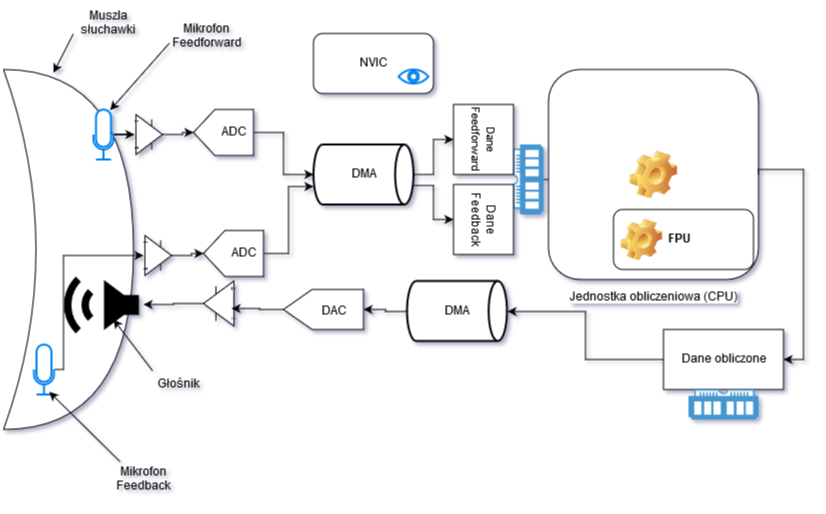
\includegraphics[width=\linewidth]{../Assets/schemat_ukladu.png}	
	\caption{Schemat układu.}
	\label{fig:schemat1}
\end{figure}
Autor pominął pomniejsze elementy, które nie wnoszą szczególnych informacji do opisu pracy. W~kwestii umiejscowienia mikrofonu odsłuchowego autor posłużył się wnioskami przedstawionymi w~artykule dotyczącym aktywnej redukcji hałasu w~zastosowaniach słuchawek tłumiących \cite{ANC4HP}. Autorzy pracy na podstawie widma częstotliwościowego wyznaczyli optymalne położenie mikrofonu i~wykazali, że takim miejscem jest bliskie otoczenie przewodu słuchowego zewnętrznego. Konkretne położenie mikrofonu odsłuchowego ilustruje lokacja nr~8 na rysunku \ref{fig:error_mic_placement} zapożyczonym z~wyżej wymienionej pracy.
Mikrofon odsłuchowy umiejscowiony w~optymalnej pozycji charakteryzuje się zlinearyzowaną odpowiedzią częstotliwościową, co ogranicza błędy pomiarowe, poprawiając precyzję zastosowanego rozwiązania.
\begin{figure}[h!]
	\centering
	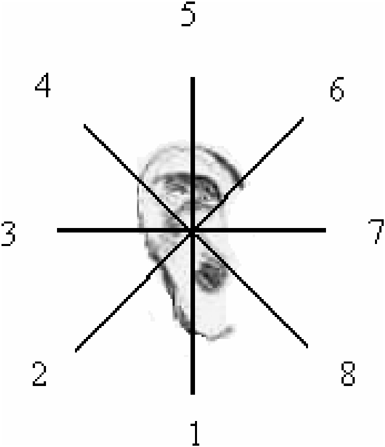
\includegraphics[scale=0.6]{../Assets/error_mic_placement.png}
	\caption{Położenie mikrofonu odsłuchowego odzwierciedla lokacja nr 8.\\ Źródło: \fullcite{ANC4HP}; strona 333}
	\label{fig:error_mic_placement}
\end{figure}

Aby stworzyć odgrodzoną przestrzeń sferyczną, autor postanowił złączyć (ścisnąć) dwie odłączone słuchawki użytych nauszników. Do celów testowych nie będzie potrzebny dodatkowy mikrofon umieszczony w~środku przestrzeni, zamiast tego zostanie użyty zamontowany już mikrofon odsłuchowy. Dane z~niego zostaną nie tylko zapisane do pamięci mikrokontrolera, ale również wysłane do komputera walidującego rozwiązanie, gdzie na bieżąco monitorowane będzie działanie układu.

Aby zasilić prototyp, autor podłączył mikrokontroler poprzez USB do komputera osobistego. Zapewniło to standardowe zasilanie mikrokontrolera na poziomie \SI{3.3}{\V}. Ponadto, celem odseparowania części analogowej od cyfrowej, autor zdecydował się zapewnić osobne zasilanie dla układów analogowych, a~więc mikrofonu wraz z~jego przedwzmacniaczem oraz dla wzmacniacza głośnikowego. Tym samym zredukowane są zakłócenia, które normalnie mogłyby się przenieść z~linii zasilania układu cyfrowego do bardzo wrażliwej na te zakłócenia części analogowej. Zasilanie to, dla mikrofonów, zostało osiągnięte poprzez dołączenie pastylkowych baterii \SI{3}{\V} typu CR2032 do elementów analogowych. Zasilanie przedwzmacniacza z~głośnikiem wymaga użycia nieco innej metody ze względu na dużą moc komponentu -- zwykła bateria nie wystarczyłaby do odpowiednio długotrwałego działania układu. Biorąc pod uwagę prototypowy charakter całego urządzenia oraz konieczność połączenia mikrokontrolera z~komputerem, autor zdecydował się zasilić przedwzmacniacz przy użyciu modułu zasilającego z~płytki prototypowej, podłączonego przez magistralę USB do komputera osobistego.